% !TEX TS-program = knitr
\documentclass[handout]{beamer}\usepackage{graphicx, color}
%% maxwidth is the original width if it is less than linewidth
%% otherwise use linewidth (to make sure the graphics do not exceed the margin)
\makeatletter
\def\maxwidth{ %
  \ifdim\Gin@nat@width>\linewidth
    \linewidth
  \else
    \Gin@nat@width
  \fi
}
\makeatother

\IfFileExists{upquote.sty}{\usepackage{upquote}}{}
\definecolor{fgcolor}{rgb}{0.2, 0.2, 0.2}
\newcommand{\hlnumber}[1]{\textcolor[rgb]{0,0,0}{#1}}%
\newcommand{\hlfunctioncall}[1]{\textcolor[rgb]{0.501960784313725,0,0.329411764705882}{\textbf{#1}}}%
\newcommand{\hlstring}[1]{\textcolor[rgb]{0.6,0.6,1}{#1}}%
\newcommand{\hlkeyword}[1]{\textcolor[rgb]{0,0,0}{\textbf{#1}}}%
\newcommand{\hlargument}[1]{\textcolor[rgb]{0.690196078431373,0.250980392156863,0.0196078431372549}{#1}}%
\newcommand{\hlcomment}[1]{\textcolor[rgb]{0.180392156862745,0.6,0.341176470588235}{#1}}%
\newcommand{\hlroxygencomment}[1]{\textcolor[rgb]{0.43921568627451,0.47843137254902,0.701960784313725}{#1}}%
\newcommand{\hlformalargs}[1]{\textcolor[rgb]{0.690196078431373,0.250980392156863,0.0196078431372549}{#1}}%
\newcommand{\hleqformalargs}[1]{\textcolor[rgb]{0.690196078431373,0.250980392156863,0.0196078431372549}{#1}}%
\newcommand{\hlassignement}[1]{\textcolor[rgb]{0,0,0}{\textbf{#1}}}%
\newcommand{\hlpackage}[1]{\textcolor[rgb]{0.588235294117647,0.709803921568627,0.145098039215686}{#1}}%
\newcommand{\hlslot}[1]{\textit{#1}}%
\newcommand{\hlsymbol}[1]{\textcolor[rgb]{0,0,0}{#1}}%
\newcommand{\hlprompt}[1]{\textcolor[rgb]{0.2,0.2,0.2}{#1}}%

\usepackage{framed}
\makeatletter
\newenvironment{kframe}{%
 \def\at@end@of@kframe{}%
 \ifinner\ifhmode%
  \def\at@end@of@kframe{\end{minipage}}%
  \begin{minipage}{\columnwidth}%
 \fi\fi%
 \def\FrameCommand##1{\hskip\@totalleftmargin \hskip-\fboxsep
 \colorbox{shadecolor}{##1}\hskip-\fboxsep
     % There is no \\@totalrightmargin, so:
     \hskip-\linewidth \hskip-\@totalleftmargin \hskip\columnwidth}%
 \MakeFramed {\advance\hsize-\width
   \@totalleftmargin\z@ \linewidth\hsize
   \@setminipage}}%
 {\par\unskip\endMakeFramed%
 \at@end@of@kframe}
\makeatother

\definecolor{shadecolor}{rgb}{.97, .97, .97}
\definecolor{messagecolor}{rgb}{0, 0, 0}
\definecolor{warningcolor}{rgb}{1, 0, 1}
\definecolor{errorcolor}{rgb}{1, 0, 0}
\newenvironment{knitrout}{}{} % an empty environment to be redefined in TeX

\usepackage{alltt}

\usetheme{Marburg}
\setbeamercovered{dynamic}
\setbeamertemplate{navigation symbols}{} 
\setbeamertemplate{footline}
{
  \leavevmode%
  \hbox{%
  \begin{beamercolorbox}[wd=.333333\paperwidth,ht=2.25ex,dp=1ex,center]{author in head/foot}%
    \usebeamerfont{author in head/foot}\copyright $\ $ \insertshortauthor%~~\beamer@ifempty{\insertshortinstitute}{}{(\insertshortinstitute)}
  \end{beamercolorbox}%
  \begin{beamercolorbox}[wd=.333333\paperwidth,ht=2.25ex,dp=1ex,center]{title in head/foot}%
    \usebeamerfont{title in head/foot} \insertinstitute
  \end{beamercolorbox}%
  \begin{beamercolorbox}[wd=.333333\paperwidth,ht=2.25ex,dp=1ex,right]{date in head/foot}%
    \usebeamerfont{date in head/foot}\insertshortdate{}\hspace*{2em}
    \insertframenumber{} / \inserttotalframenumber\hspace*{2ex} 
  \end{beamercolorbox}}%
  \vskip0pt%
}

\usepackage{amsmath}
\usepackage{caption}
\usepackage{color}
\usepackage{enumerate}
\usepackage{listings}
\usepackage{hyperref}
\usepackage{mathrsfs}
\usepackage{natbib}
\usepackage{url}

\providecommand{\all}{\ \forall \ }
\providecommand{\bs}{\backslash}
\providecommand{\e}{\varepsilon}
\providecommand{\E}{\ \exists \ }
\providecommand{\lm}[2]{\lim_{#1 \rightarrow #2}}
\providecommand{\m}[1]{\mathbb{#1}}
\providecommand{\nv}{{}^{-1}}
\providecommand{\ov}[1]{\overline{#1}}
\providecommand{\p}{\newpage}
\providecommand{\q}{$\quad$ \newline}
\providecommand{\rt}{\rightarrow}
\providecommand{\Rt}{\Rightarrow}
\providecommand{\vc}[1]{\boldsymbol{#1}}
\providecommand{\wh}[1]{\widehat{#1}}

\hypersetup{colorlinks,linkcolor=,urlcolor=blue}
\numberwithin{equation}{section}

\definecolor{dkgreen}{rgb}{0,0.6,0}
\definecolor{gray}{rgb}{0.5,0.5,0.5}
\definecolor{mauve}{rgb}{0.58,0,0.82}

\lstset{ 
  language=C,                % the language of the code
  basicstyle= \footnotesize,           % the size of the fonts that are used for the code
  numberstyle= \tiny \color{white},  % the style that is used for the line-numbers
  stepnumber=2,                   % the step between two line-numbers. 
  numbersep=5pt,                  % how far the line-numbers are from the code
  backgroundcolor=\color{white},      % choose the background color. You must add \usepackage{color}
  showspaces=false,               % show spaces adding particular underscores
  showstringspaces=false,         % underline spaces within strings
  showtabs=false,                 % show tabs within strings adding particular underscores
  frame=lrb,                   % adds a frame around the code
  rulecolor=\color{black},        % if not set, the frame-color may be changed on line-breaks within not-black text 
  tabsize=2,                      % sets default tabsize to 2 spaces
  captionpos=t,                   % sets the caption-position 
  breaklines=true,                % sets automatic line breaking
  breakatwhitespace=false,        % sets if automatic breaks should only happen at whitespace
  %title=\lstname,                   % show the filename of files included with \lstinputlisting;
  keywordstyle=\color{blue},          % keyword style
  commentstyle=\color{gray},       % comment style
  stringstyle=\color{dkgreen},         % string literal style
  escapeinside={\%*}{*)},            % if you want to add LaTeX within your code
  morekeywords={*, ...},               % if you want to add more keywords to the set
  xleftmargin=0.053in, % left horizontal offset of caption box
  xrightmargin=-.03in % right horizontal offset of caption box
}

%\DeclareCaptionFont{white}{\color{white}}
%\DeclareCaptionFormat{listing}{\parbox{\textwidth}{\colorbox{gray}{\parbox{\textwidth}{#1#2#3}}\vskip-0.05in}}
%\captionsetup[lstlisting]{format = listing, labelfont = white, textfont = white}
%For caption-free listings, comment out the 3 lines above and uncomment the 2 lines below.
 \captionsetup{labelformat = empty, labelsep = none}
 \lstset{frame = single}





\title{Describing Relationships Between Variables (Ch. 4)}
\author{Will Landau}
\date{\today}
\institute{Iowa State University}

\begin{document}

\begin{frame}
\titlepage
\end{frame}
 
 \AtBeginSection[]
{
   \begin{frame}
       \frametitle{Outline}
       \tableofcontents[currentsection]
   \end{frame}
}

\section{Introduction}

\begin{frame}[fragile]
\frametitle{\small Pressing pressures and specimen densities for a ceramic compound}
\scriptsize
A mixture of $\text{Al}_2\text{O}_3$, polyvinyl alcohol, and water was prepared, dried overnight, crushed, and sieved to obtain 100 mesh size grains. These were pressed into cylinders at pressures from 2,000 psi to 10,000 psi, and cylinder densities were calculated. 

% latex table generated in R 2.15.3 by xtable 1.7-1 package
% Thu Apr 11 22:14:01 2013
\begin{table}[ht]
\centering
\begin{tabular}{rr}
 x (pressure in psi) & y (density in g/cc) \\ 
  \hline
2000.00 & 2.49 \\ 
  2000.00 & 2.48 \\ 
  2000.00 & 2.47 \\ 
  4000.00 & 2.56 \\ 
  4000.00 & 2.57 \\ 
  4000.00 & 2.58 \\ 
  6000.00 & 2.65 \\ 
  6000.00 & 2.66 \\ 
  6000.00 & 2.65 \\ 
  8000.00 & 2.72 \\ 
  8000.00 & 2.77 \\ 
  8000.00 & 2.81 \\ 
  10000.00 & 2.86 \\ 
  10000.00 & 2.88 \\ 
  10000.00 & 2.86 \\ 
  \end{tabular}
\end{table}



\end{frame}

\begin{frame}[fragile]
\frametitle{\small Scatterplot: ceramics data}

\begin{center}
\begin{knitrout}
\definecolor{shadecolor}{rgb}{0.969, 0.969, 0.969}\color{fgcolor}
\includegraphics[width=.8\textwidth,height=.6\textheight]{figure/unnamed-chunk-3} 

\end{knitrout}

\end{center}
\end{frame}


\begin{frame}[fragile]
\frametitle{}
\begin{center}
\begin{knitrout}
\definecolor{shadecolor}{rgb}{0.969, 0.969, 0.969}\color{fgcolor}
\includegraphics[width=.8\textwidth,height=.6\textheight]{figure/unnamed-chunk-4} 

\end{knitrout}

\end{center}

\begin{itemize}
\item The line,  $y \approx 2.375 + 4.867 \times 10^{-5} x$, is the {\bf regression line} fit to the data.
\end{itemize}
\end{frame}

\begin{frame}
\frametitle{Why fit a regression line?}
\begin{enumerate}[1. ]
\pause \item To predict future values of $y$ based on $x$.
\begin{itemize}
\pause \item I.e., a new ceramic under pressure $x = 5000$ psi should have a density of $2.375 + 4.867 \times 10^{-5} \cdot 5000 = 2.618$ g/cc. 
\end{itemize}
\pause \item To characterize the relationship between $x$ and $y$ in terms of strength, direction, and shape.
\begin{itemize}
\pause \item In the ceramics data, density has a strong, positive, linear association with $x$. 
\pause \item On average, the density increases by $4.867 \times 10^{-5}$ g/cc for every increase in pressure of 1 psi.
\end{itemize}
\end{enumerate}
\end{frame}

\section{Fitting a regression line}

\begin{frame}
\frametitle{Fitting a linear regression line}
\begin{itemize}
\pause \item For a response variable $y$ and a predictor variable $x$, we declare:
\pause \begin{align*}
y \approx b_0 + b_1 x
\end{align*}
\pause \item and then calculate the intercept $b_0$ and slope $b_1$ using {\bf least squares}.
\begin{itemize}
\pause \item We apply the {\bf principle of least squares}: that is, the best-fit line is given by minimizing the {\bf loss function} in terms of $b_0$ and $b_1$:
\pause \begin{align*}
S(b_0, b_1) = \sum_{i = 1}^n (y_i - \wh{y}_i)^2
\end{align*} 
\pause \item Here, $\wh{y}_i  = b_0 + b_1 x_i$
\end{itemize}
\end{itemize}
\end{frame}


\begin{frame}
\frametitle{\small Minimize $\sum_{i = 1}^n (y_i - \wh{y}_i)^2$ to get the line as close as possible to the points.}
\setkeys{Gin}{width=1\textwidth} 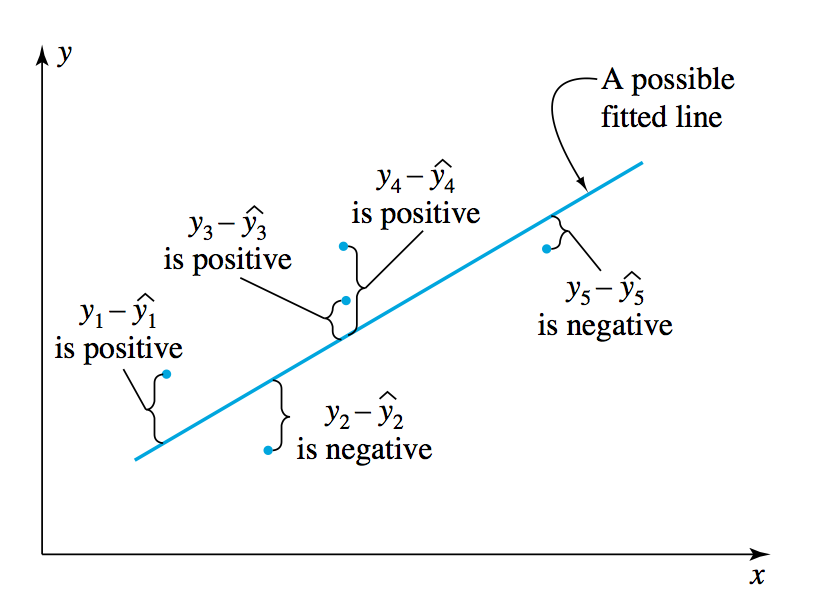
\includegraphics{../../fig/lossfunplot.png}
\end{frame}


\begin{frame}
\frametitle{How to apply least squares to get the regression line}
\begin{itemize}
\pause \item From the principle of least squares, one can derive the {\bf normal equations}:
\begin{align*}
\uncover<2->{n b_0 + b_1 \sum_{i = 1}^n x_i} &= \uncover<2->{\sum_{i = 1}^n y_i} \\
\uncover<3->{b_0 \sum_{i = 1}^n x_i + b_1 \sum_{i = 1}^n x_i^2} &= \uncover<3->{\sum_{i = 1}^n x_i y_i}
\end{align*}
\pause \pause \item and then solve for $b_0$ and $b_1$:
\begin{align*}
\color{blue} \uncover<5->{b_1 = \frac{\sum(x_i - \ov{x})(y_i - \ov{y})}{\sum(x_i - \ov{x})^2}} \qquad \uncover<6->{b_0 = \ov{y}- b_1 \ov{x}}
\end{align*}
\end{itemize}
\end{frame}

\begin{frame}[fragile]
\frametitle{Example: plastics hardness data} \small
Eight batches of plastic are made. From each batch one test item is molded. At a given time (in hours), it hardness is measured in units (assume freshly-melted plastic has a hardness of 0 units). The following are the 8 measurements and times.

\begin{minipage}[b]{0.47\linewidth} 
% latex table generated in R 2.15.3 by xtable 1.7-1 package
% Thu Apr 11 22:14:02 2013
\begin{table}[ht]
\centering
\begin{tabular}{rr}
 time & hardness \\ 
  \hline
32.00 & 230.00 \\ 
  72.00 & 323.00 \\ 
  64.00 & 298.00 \\ 
  48.00 & 255.00 \\ 
  16.00 & 199.00 \\ 
  40.00 & 248.00 \\ 
  80.00 & 359.00 \\ 
  56.00 & 305.00 \\ 
  \end{tabular}
\end{table}


\end{minipage}
\begin{minipage}[b]{0.47\linewidth} 
\begin{knitrout}
\definecolor{shadecolor}{rgb}{0.969, 0.969, 0.969}\color{fgcolor}
\includegraphics[width=\maxwidth]{figure/unnamed-chunk-6} 

\end{knitrout}

\end{minipage}

\end{frame}

\begin{frame}[fragile]
\frametitle{Fitting the line} \scriptsize
\begin{itemize}
\pause \item $\ov{x} = 51$
\pause \item $\ov{y} = 277.125$ \pause
% latex table generated in R 2.15.3 by xtable 1.7-1 package
% Thu Apr 11 22:14:02 2013
\begin{table}[ht]
\centering
\begin{tabular}{rrrrrr}
 x & y & $x_i - \ov{x}$ & $y_i - \ov{y}$ & $(x_i - \ov{x})(y_i - \ov{y})$ & $(x_i - \ov{x})^2$ \\ 
  \hline
32.00 & 230.00 & -19.00 & -47.12 & 895.38 & 361.00 \\ 
  72.00 & 323.00 & 21.00 & 45.88 & 963.38 & 441.00 \\ 
  64.00 & 298.00 & 13.00 & 20.88 & 271.38 & 169.00 \\ 
  48.00 & 255.00 & -3.00 & -22.12 & 66.38 & 9.00 \\ 
  16.00 & 199.00 & -35.00 & -78.12 & 2734.38 & 1225.00 \\ 
  40.00 & 248.00 & -11.00 & -29.12 & 320.38 & 121.00 \\ 
  80.00 & 359.00 & 29.00 & 81.88 & 2374.38 & 841.00 \\ 
  56.00 & 305.00 & 5.00 & 27.88 & 139.38 & 25.00 \\ 
  \end{tabular}
\end{table}


\pause \item $\sum (x_i - \ov{x})(y_i - \ov{y}) = 895.38 +  963.38  + \cdots  139.38  =  7765 $
\pause \item $\sum (x_i - \ov{x})^2= 361 +  441  + \cdots  25  =  3192 $
\pause \item $b_1 = \frac{7765}{3192} = 2.43$
\pause \item $b_0 = \ov{y} - b_1 \ov{x} = 277.125 - 2.43 \cdot 51 = 153.19$
\end{itemize}
\end{frame}


\begin{frame}[fragile]
\frametitle{Plot the line to check the fit.} \small
\begin{center}
\begin{knitrout}
\definecolor{shadecolor}{rgb}{0.969, 0.969, 0.969}\color{fgcolor}
\includegraphics[width=0.8\textwidth,height=0.8\textheight]{figure/unnamed-chunk-8} 

\end{knitrout}


\end{center}
\end{frame}

\begin{frame}
\frametitle{Interpret the model terms}
\begin{itemize}
\pause \item $b_1 = 2.43$ means that on average, the plastic hardens 2.43 more units for every additional hour it is allowed to harden.
\pause \item $b_0 = 153.19$ means that at the very beginning of the hardening process (time = 0 hours), the plastics had a hardness of 153.19 on average, IF the model is still correct around time 0.
\begin{itemize}
\pause \item But we know that the plastics were completely molten at the very beginning, with a hardness of 0.
\pause \item Don't {\bf extrapolate}: i.e., predict $y$ values beyond the range of the $x$ data.
\end{itemize}
\end{itemize}
\end{frame}

\begin{frame}
\frametitle{Checking a fitted line}

\begin{enumerate}[1. ]
\pause \item Is the model useful?
\begin{itemize}
\pause \item How closely do the points cluster around the line?
\pause \item How strong is the linear relationship between $x$ and $y$?
\pause \item How much variation in $y$ can be explained by the fitted line?  
\pause \item How well can the fitted line predict future values of $y$?
\pause \item Is the model \emph{precise}?
\end{itemize}
\pause \item Is the model valid?
\begin{itemize}
\pause \item Should we really be using a straight line to explain $y$ using $x$, or would some other equation (like a parabola) be better?
\pause \item Does $y$ deviate from the fitted line in some systematic way?
\pause \item Is the model \emph{valid}?
\end{itemize}
\end{enumerate}
\end{frame}


\section{Is the model useful?}

\begin{frame}
\frametitle{Linear correlation: a measure of the usefulness of a fitted line}
\begin{itemize}
\pause \item {\bf Linear correlation}:
\pause \begin{align*}
r = \frac{\sum(x_i - \ov{x})(y_i - \ov{y})}{\sqrt{\sum (x_i - \ov{x})^2 \sum (y_i - \ov{y})^2}}
\end{align*}
\pause \item As it turns out:
\pause \begin{align*}
r = b_1\frac{s_x}{s_y}
\end{align*}
\pause where $s_x$ is the standard deviation of the $x_i$'s and $x_y$ is the standard deviation of the $y_i$'s. 
\end{itemize}
\end{frame}

\begin{frame}
\frametitle{Facts about linear correlation}
\begin{itemize}
\pause \item $-1 \le r \le 1$
\pause \item $r < 0$ means a negative slope, $r > 0$ means a positive slope
\pause \item High $|r|$ means $x$ and $y$ have a strong linear relationship (high correlation), and low $|r|$ implies a weak linear relationship (low correlation).
\end{itemize}

\setkeys{Gin}{width=1\textwidth} 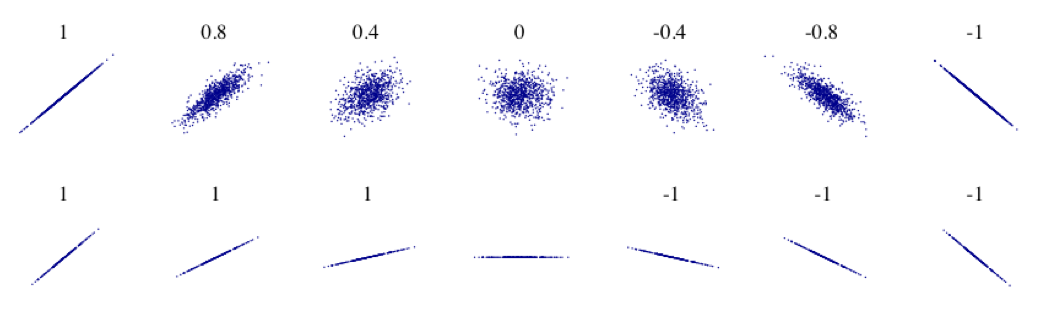
\includegraphics{../../fig/diffcorrs.png}
\end{frame}

\begin{frame}[fragile]
\frametitle{Correlation in the ceramics data}
\begin{center}
\begin{knitrout}
\definecolor{shadecolor}{rgb}{0.969, 0.969, 0.969}\color{fgcolor}
\includegraphics[width=.8\textwidth,height=.6\textheight]{figure/unnamed-chunk-9} 

\end{knitrout}

\end{center}
\begin{itemize}
\pause \item $s_x = 2927.7002$, $s_y= 0.1438$  $b_1 = 4.867 \cdot 10^{-5}$
\pause \item $r = b_1 \frac{s_x}{s_y} $  = \ensuremath{4.867\times 10^{-5}} $\frac{2927.7002}{0.1438}$ = 0.9911
\end{itemize}

\end{frame}

\begin{frame}[fragile]
\frametitle{Correlation in the plastics data} \scriptsize
\begin{itemize}
\pause \item $\ov{x} = 51$
\pause \item $\ov{y} = 277.125$ \pause 
% latex table generated in R 2.15.3 by xtable 1.7-1 package
% Thu Apr 11 22:14:02 2013
\begin{table}[ht]
\centering
\begin{tabular}{rrrrrrr}
 x & y & $x_i - \ov{x}$ & $y_i - \ov{y}$ & $(x_i - \ov{x})^2$ & $(y_i - \ov{y})^2$ & $\Delta x \Delta y$ \\ 
  \hline
32.00 & 230.00 & -19.00 & -47.12 & 361.00 & 2220.77 & 895.38 \\ 
  72.00 & 323.00 & 21.00 & 45.88 & 441.00 & 2104.52 & 963.38 \\ 
  64.00 & 298.00 & 13.00 & 20.88 & 169.00 & 435.77 & 271.38 \\ 
  48.00 & 255.00 & -3.00 & -22.12 & 9.00 & 489.52 & 66.38 \\ 
  16.00 & 199.00 & -35.00 & -78.12 & 1225.00 & 6103.52 & 2734.38 \\ 
  40.00 & 248.00 & -11.00 & -29.12 & 121.00 & 848.27 & 320.38 \\ 
  80.00 & 359.00 & 29.00 & 81.88 & 841.00 & 6703.52 & 2374.38 \\ 
  56.00 & 305.00 & 5.00 & 27.88 & 25.00 & 777.02 & 139.38 \\ 
  \end{tabular}
\end{table}


\pause \item $\sum (x_i - \ov{x})(y_i - \ov{y}) = 895.39 + 963.38 + \cdots + 139.38 = 7765$
\pause \item $\sum (x_i - \ov{x})^2 = 361 + 441 + \cdots + 25 = 3192$
\pause \item $\sum (y_i - \ov{y})^2 = 2220.77 + 2104.52 + \cdots + 777.02 = $ \ensuremath{1.9683\times 10^{4}}
\pause \item $r = \frac{ (x_i - \ov{x})(y_i - \ov{y})  }{\sqrt{  (x_i - \ov{x})^2   (y_i - \ov{y})^2  }} = \frac{7765}{\sqrt{3192 \cdot 1.9683 \times 10^4}} = $ 0.9796
\end{itemize}
\end{frame}

\begin{frame}
\frametitle{\small CAUTION: the data may be highly correlated even if the \emph{linear} correlation, $r$, is low.}
\setkeys{Gin}{width=1\textwidth} 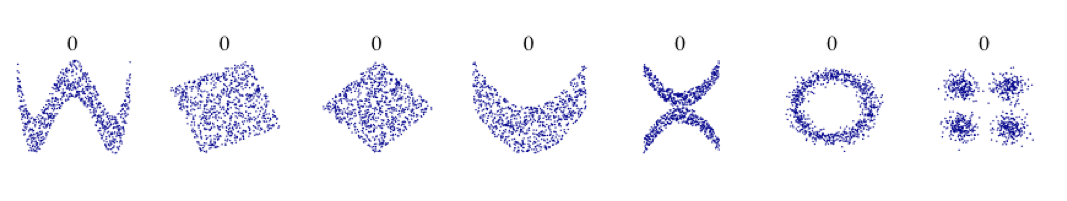
\includegraphics{../../fig/corr0.png}
\end{frame}


\begin{frame}
\frametitle{Coefficient of determination} \scriptsize
\begin{itemize}
\pause \item {\bf Coefficient of determination}: another measure of the usefulness of a fitted line, defined by:
\pause \begin{align*}
R^2 = \frac{\sum(y_i - \ov{y})^2 - \sum(y_i - \wh{y}_i)^2}{\sum(y_i - \ov{y})^2}
\end{align*}
\pause where $y_i = b_0 + b_1 x_i$. 
\pause \item Fortunately,
\begin{align*} \color{blue}
R^2 = r^2
\end{align*}
\pause \item Interpretation: $R^2$ is the fraction of variation in the response variable ($y$) explained by the fitted line.
\pause \item Ceramics data: $R^2 = r^2 = 0.9911^2 = 0.9823$, so  98.23\% of the variation in density is explained by a linear equation in terms of pressure. Hence, the line is useful for predicting density from pressure.
\pause \item Plastics data: $R^2 = r^2 = 0.9796^2 = 0.9596$, so  95.96\% of the variation in hardness is explained by a linear equation in terms of time. Hence, so the line is useful for predicting hardness from time.

\end{itemize}
\end{frame}


\begin{frame}[fragile]
\frametitle{\small $R^2$ measures \emph{usefulness} (or precision), not validity.}
\begin{center}
\begin{itemize}
\item $x$ and $y$ can have a true linear relationship despite a low $R^2$
\end{itemize}
\begin{knitrout}
\definecolor{shadecolor}{rgb}{0.969, 0.969, 0.969}\color{fgcolor}
\includegraphics[width=.6\textwidth,height=.6\textheight]{figure/unnamed-chunk-11} 

\end{knitrout}

\end{center}
\begin{itemize}
\item $R^2 = $ 0.4832
\end{itemize}
\end{frame}



\section{Is the model valid?}

\begin{frame}[fragile]
\frametitle{\small CAUTION: Sometimes, the true relationship between $x$ and $y$ is not linear, despite a high $R^2$}
\begin{center}
\begin{knitrout}
\definecolor{shadecolor}{rgb}{0.969, 0.969, 0.969}\color{fgcolor}
\includegraphics[width=.6\textwidth,height=.6\textheight]{figure/unnamed-chunk-12} 

\end{knitrout}

\end{center}
\begin{itemize}
\item $R^2 = $ 0.9796
\end{itemize}
\end{frame}


\begin{frame}
\frametitle{\small Residuals: a way to check the validity of a fitted line}
\begin{itemize}
\pause \item {\bf Residuals}: numbers $e_i$ of the form: 
\begin{align*}
\uncover<2->{e_i} &\uncover<2->{= y_i - \wh{y_i}}  \\
&\uncover<3->{=  y_i - (b_0 + b_1 x_i)}
\end{align*}
\pause \pause \item Instead of:
\begin{align*}
y_i &\approx b_0 + b_1 x_i
\intertext{\uncover<5->{or:}}
\uncover<5->{\wh{y_i}} &\uncover<5->{=b_0 + b_1 x_i}
\intertext{\uncover<6->{you can now write:}}
\uncover<6->{y_i} &\uncover<6->{= b_0 + b_1 x_i + e_i}
\end{align*}
\end{itemize}
\end{frame}

\begin{frame}
\frametitle{\small What do residuals mean? (Scatterplot: heights and weights of 10 elderly men)}
\begin{center}
\setkeys{Gin}{width=.6\textwidth} 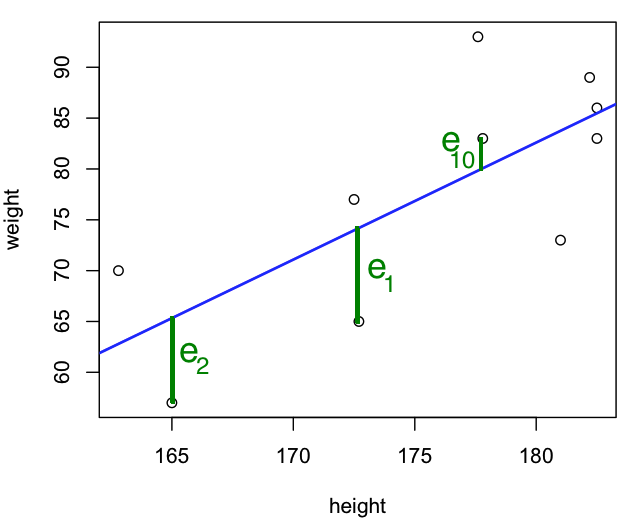
\includegraphics{../../fig/residmeaning}
\end{center}
\begin{itemize}
\item Residuals are the vertical distances between the points and the fitted line.
\end{itemize}
\end{frame}

\begin{frame}[fragile]
\frametitle{Residuals: heights and weights of elderly men data}
% latex table generated in R 2.15.3 by xtable 1.7-1 package
% Thu Apr 11 22:14:03 2013
\begin{table}[ht]
\centering
\begin{tabular}{rrrr}
 $x_i$ (height in cm) & $y_i$ (weight in kg) & $\wh{y}_i$ & $e_i = y_i - \wh{y}_i$ \\ 
  \hline
172.70 & 65.00 & 74.19 & -9.19 \\ 
  165.00 & 57.00 & 65.32 & -8.32 \\ 
  172.50 & 77.00 & 73.96 & 3.04 \\ 
  182.20 & 89.00 & 85.13 & 3.87 \\ 
  177.60 & 93.00 & 79.83 & 13.17 \\ 
  181.00 & 73.00 & 83.75 & -10.75 \\ 
  182.50 & 83.00 & 85.48 & -2.48 \\ 
  182.50 & 86.00 & 85.48 & 0.52 \\ 
  162.80 & 70.00 & 62.79 & 7.21 \\ 
  177.80 & 83.00 & 80.06 & 2.94 \\ 
  \end{tabular}
\end{table}


\end{frame}

\begin{frame}[fragile]
\frametitle{\small Plots of residuals} \scriptsize
\begin{center}
\begin{knitrout}
\definecolor{shadecolor}{rgb}{0.969, 0.969, 0.969}\color{fgcolor}
\includegraphics[width=0.6\textwidth,height=.35\textheight]{figure/unnamed-chunk-14} 

\end{knitrout}

\begin{knitrout}
\definecolor{shadecolor}{rgb}{0.969, 0.969, 0.969}\color{fgcolor}
\includegraphics[width=0.6\textwidth,height=.35\textheight]{figure/unnamed-chunk-15} 

\end{knitrout}

\end{center}

The model fits well since there is no discernible pattern in the residuals when plotted.
\end{frame}

\begin{frame}
\frametitle{\small Residual plots and validity}
\begin{itemize}
\pause \item Left: data that don't fit a line
\pause \item Right: the plot of residuals on $x$
\begin{itemize}
\pause \item The residuals show a nonlinear pattern in the residual plot.
\pause \item Hence, the fitted line is not a valid model.
\end{itemize}
\end{itemize}
\setkeys{Gin}{width=1\textwidth} 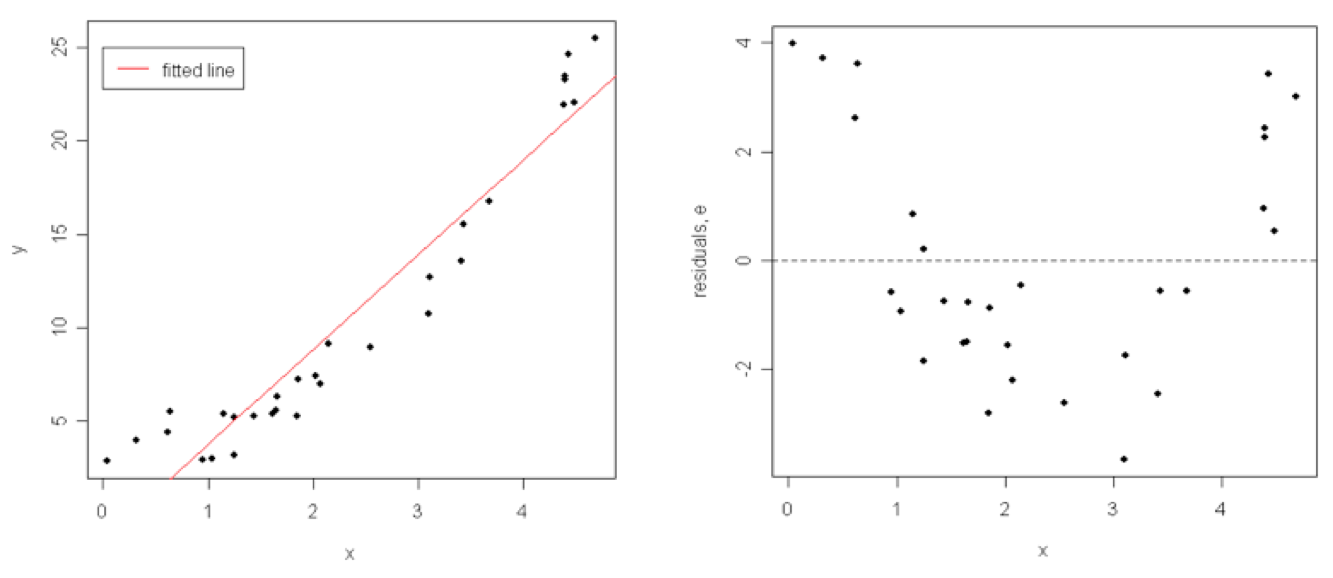
\includegraphics{../../fig/residbad.png}
\end{frame}

\begin{frame}
\frametitle{\small More residual plots and patterns} \scriptsize
\begin{itemize}
\pause \item All patterns are bad in plots of residual vs. fitted values, $x$, time, etc.
\begin{center}
\setkeys{Gin}{width=.75\textwidth} \includegraphics<2->{../../fig/residpatterns.png}
\end{center}
\pause \pause \item When we get to inference, we want to make sure the residuals have a bell-shaped distribution:
\begin{center}
\setkeys{Gin}{width=.4\textwidth}  \includegraphics<4->{../../fig/residqqnorm.png}
\end{center}
\pause \item This normal QQ plot shows that the residuals are roughly bell-shaped, which is good.
\end{itemize}

\end{frame}


\end{document}
